\documentclass{beamer}
\documentclass[norsk,a4paper,12pt]{article}
\usepackage[utf8]{inputenc}
\usepackage[english]{babel}
\usepackage{csquotes}	% Supports babel
\usepackage{fancyhdr}
\usepackage{graphicx} %for å inkludere grafikk
\usepackage{verbatim} %for å inkludere filer med tegn LaTeX ikke liker
\usepackage{tabularx}
\usepackage{booktabs}
\usepackage{amsmath}
\usepackage{float}
\usepackage{color}
\usepackage{xcolor}
\usepackage{listings}
\usepackage{hyperref}
\usepackage{amsmath}
\usepackage{tikz}
\usepackage{physics}	% Dirac notation
\usepackage{amssymb}
\usepackage{titlesec}
\usepackage{comment}
\usepackage{fancybox}	% Oval equation box
\usepackage{enumitem}	% Itemize settings
\usepackage{subfig}		% Sub figures
\usepackage{subfloat}	% Figures side by side
\usepackage{geometry}	% Change margins on each page
\usepackage{empheq}		% Beautiful boxes
\usepackage{multirow}	% Multirow in table
\usepackage{multicol}	% Multicolumn in table
\usepackage{varwidth}	% Rotate text in table
\usepackage{arydshln}   % Dashed lines in table

%biblatex
\usepackage[
backend=bibtex,
style=alphabetic,
sorting=ynt
]{biblatex}
\addbibresource{refs.bib}

%listings
\lstset{language=c++}
\lstset{basicstyle=\small}
\lstset{backgroundcolor=\color{white}}
\lstset{frame=single}
\lstset{stringstyle=\ttfamily}
\lstset{keywordstyle=\color{red}\bfseries}
\lstset{commentstyle=\itshape\color{blue}}
\lstset{showspaces=false}
\lstset{showstringspaces=false}
\lstset{showtabs=false}
\lstset{breaklines}
\lstset{postbreak=\raisebox{0ex}[0ex][0ex]{\ensuremath{\color{red}\hookrightarrow\space}}}

%tikz
\setcounter{secnumdepth}{4}
\usetikzlibrary{through, shapes, calc, shapes, arrows, positioning, arrows.meta, shadows}
\tikzstyle{neuron}=[draw,circle,minimum size=20pt,inner sep=0pt, fill=white]
\tikzstyle{stateTransition}=[thick]
\tikzstyle{learned}=[text=red]

%\newcommand{\blds}[1]{\boldsymbol{{#1}}} % better bold in mathmode (from amsmath)
%\newcommand{\Arf}[1]{\Autoref{#1}}
%\renewcommand\normalfont\huge\bfseries\scshape\color{ForestGreen}

%specific reused text
\newcommand{\mdate}{\today}
\newcommand{\mtitle}{Solving Many-body Quantum Problem using Machine Learning}
\newcommand{\mauthor}{Even Marius Nordhagen}
\newcommand{\massignn}{.}

\newcommand{\prtl}{\mathrm{\partial}} %reduce length of partial (less to write)
% \NewDocumentCommand{\prd}{m O{} O{}}{\frac{\prtl^{#3}{#2}}{\prtl{#1}^{#3}}}
\newcommand{\prdp}[2]{\left(\frac{\prtl}{\prtl #1}\right)^{#2}}
\newcommand{\vsp}{\vspace{0.15cm}} %small vertical space
\newcommand{\txtit}[1]{\textit{{#1}}} %italic text
\newcommand{\blds}[1]{\boldsymbol{{#1}}} % better bold in mathmode (from amsmath)
\newcommand{\bigO}{\mathcal{O}} %nice big O
\newcommand{\me}{\mathrm{e}} %straight e for exp
\newcommand{\md}{\mathrm{d}} %straight d for differential
\newcommand{\mRe}[1]{\mathrm{Re}\left({#1}\right)}%nice real
\newcommand{\munit}[1]{\;\ensuremath{\, \mathrm{#1}}} %straight units in math
\newcommand{\Rarr}{\Rightarrow} %reduce lenght of Rightarrow (less to write)
\newcommand{\rarr}{\rightarrow} %reduce lenght of rightarrow (less to write)
\newcommand{\ecp}[1]{\left< {#1} \right>} %expected value
\newcommand{\urw}{\uparrow} % up arrow
\newcommand{\drw}{\downarrow} % down arrow
\newcommand{\pt}[1]{\textbf{\txtit{#1}}\justify}
\newcommand{\infint}{\int\limits^{\infty}_{-\infty}}
\newcommand{\oinfint}{\int\limits^{\infty}_0}
\newcommand{\sint}{\int\limits^{2\pi}_0\int\limits^{\pi}_0\oinfint}
\newcommand{\arcsinh}[1]{\text{arcsinh}\left(#1\right)}
\newcommand{\I}{\scalebox{1.2}{$\mathds{1}$}}
\newcommand{\veps}{\varepsilon} %\varepsilon is to long :P
\newcommand{\cnj}[1]{{#1}^{*}}
\newcommand{\Arf}[1]{\Autoref{#1}}
\newcommand{\suml}[2]{\sum\limits^{#2}_{#1}}
\newcommand{\sumll}[1]{\sum\limits_{#1}}
\newcommand{\tsup}[1]{\textsuperscript{#1}}
\newcommand{\wtld}[1]{\widetilde{#1}}

\newcommand{\ufij}[3]{#1_{#2\rarr#3}}
\newcommand{\Ham}{\hat{H}}
\newcommand{\mb}[1]{\blds{#1}}
\newcommand{\psiTcnj}{\cnj{\Psi}_T(\mb{R};\mb{\alpha})}
\newcommand{\psiT}{{\Psi}_T(\mb{R};\mb{\alpha})}
\newcommand{\phiT}{{\Phi}_T(\mb{R};\mb{\alpha})}
\newcommand{\dinner}[2]{\bra{#1}#2\ket{#1}}
\newcommand{\pinner}{\dinner{\Psi_T}{}}
\newcommand{\langevin}{\prd{t}[r] = DF(r(t)) + \eta}
\newcommand{\rnew}{r^{\text{new}}}
\newcommand{\rold}{r^{\text{old}}}
\newcommand{\Fnew}{F^{\text{new}}}
\newcommand{\Fold}{F^{\text{old}}}
\newcommand{\FokkerPlanck}{\prd{t}[P] = \sum_i D\prd{x_i}\left(\prd{x_i} - \mb{F_i}\right)P}
\newcommand{\Kin}{\frac{1}{2}\sum_i\nabla^2_i}
\newcommand{\frij}{f(\blds{r}_i, \blds{r}_j)}
\newcommand{\fij}{f_{ij}}
\newcommand{\HO}{V(\blds{R}) - \Kin}
\newcommand{\HI}{\sum\limits_{i<j} \frij}
\newcommand{\EHF}{E\left[\Psi^{\text{HF}}\right]}
\newcommand{\HIinnerAS}[2]{\bra{\psi_{#1}\psi_{#2}}H_I\ket{\psi_{#1}\psi_{#2}} - \bra{\psi_{#1}\psi_{#2}}H_I\ket{\psi_{#2}\psi_{#1}}}

\newcommand{\ijnorm}[2]{\sqrt{\braket{#1}{#1}\braket{#2}{#2}}}
\newcommand{\twoDI}{I_{\text{2D}}}
\newcommand{\sumE}[3]{\suml{#1}{#2+#3} E^{#2#3}_{#1}}

\newcommand\CC{C\nolinebreak[4]\hspace{-0.01em}\raisebox{.3ex}{\relsize{-1.35}{\textbf{++}}}\;}
\newcommand{\pp}[1]{#1\nolinebreak[4]\hspace{-.01em}\raisebox{.25ex}{\relsize{-1.5}{\textbf{++}}}\;}

\newcommand{\psiDW}{\psi^{\text{DW}}}
\newcommand{\psiHO}{\psi^{\text{HO}}}
\newcommand{\hDW}{h^{\text{DW}}}
\newcommand{\VDW}{V^{\text{DW}}}
\newcommand{\VHO}{V^{\text{HO}}}
\newcommand{\UDW}{U^{\text{DW}}}

% Define new column alignment types
\newcolumntype{L}[1]{>{\raggedright\let\newline\\\arraybackslash\hspace{0pt}}m{#1}}
\newcolumntype{R}[1]{>{\raggedleft\let\newline\\\arraybackslash\hspace{0pt}}m{#1}}
\newcolumntype{C}{>{\centering\let\newline\\\arraybackslash\hspace{0pt}}X}

% OWN DEFS
\newcommand{\bs}[1]{\boldsymbol{{#1}}}
\newcommand{\detup}{\det(\hat{D}^{\uparrow})}
\newcommand{\detdn}{\det(\hat{D}^{\downarrow})}
\newcommand{\hatH}{\hat{\text{H}}}
\newcommand{\psin}{\Psi_n(\bs{r})}
\newcommand{\psinc}{\Psi_n^*(\bs{r})}
\newcommand{\VMC}{Variational Monte Carlo}
\newcommand{\hatT}{\hat{T}}
\newcommand{\detD}{|\hat{D}|}
\pagestyle{fancy}

\author{Even Marius Nordhagen} 
\institute[UiO] { University of Oslo \\ 
                  \medskip
                  \textit{evenmn@fys.uio.no}
                }
\date{\today} 
\title{Studies of Quantum Dots using Machine Learning}

\begin{document}

\frontframe

\mframe{Outline}{
\begin{itemize}
	\item Motivation
	\item Quantum Theory
	\item Machine Learning
	\item Methods
	\item Results
	\item Conclusion
	\item (Code)
\end{itemize}
}

\titleframe{Motivation}

\mframe{Why quantum dots?}{
	\begin{itemize}
		\item Technology \supercite{noauthor_samsung_nodate}
		\item Theoretically
		\item Experimentally (2D)
	\end{itemize}
}

\mframe{Why is it challenging?}{
	\begin{itemize}
		\item Quantum many-body problem
		\item Fermi-Dirac statistics
	\end{itemize}
}

\mframe{How to overcome the challenges?}{
	\begin{itemize}
		\item Efforts..
		\item gh
		\item Our approach: Machine Learning \supercite{carleo_solving_2017, pfau2019abinitio}
	\end{itemize}
}

\titleframe{Quantum Theory}

\mframe{The Time-independent Schrödinger Equation}{
A stationary quantum mechanical system is described by 
	\begin{equation}
	E_n=\frac{\int d\bs{R}\psinc\hat{\mathcal{H}}\psin}{\int d\bs{R}\psinc\psin}
	\end{equation}
which gives the energy of state $n$.
}

\iffalse
\mframe{Harmonic Oscillator}{

\begin{equation}
\begin{aligned}
\hat{\mathcal{H}} &= -\frac{1}{2}\nabla^2 + \frac{1}{2} \omega^2r^2\\
&= \langle\hat{T}\rangle + \langle\hat{V}\rangle
\end{aligned}
\end{equation}

\begin{figure}
	\centering
	\begin{tikzpicture}
\begin{axis}[domain=-3.5:3.5, samples=50,no markers, hide axis,y=1cm,thick]
\addplot [gray] {0.5*x^2};
\node[label={180:{(-2,2)}},circle,fill,inner sep=2pt] at (axis cs:-2,2) {};
\end{axis}
\end{tikzpicture}
\end{figure}

}

\mframe{Circular Quantum Dots}{
	\begin{equation}
	\begin{aligned}
	\hat{\mathcal{H}} &= -\frac{1}{2}\nabla_1^2 -\frac{1}{2}\nabla_2^2 + \frac{1}{2} \omega^2r_1^2 + \frac{1}{2} \omega^2r_2^2 + \frac{1}{r_{ij}}\\
	&= \langle\hat{T}_1\rangle + \langle\hat{T}_2\rangle + \langle\hat{V}_1\rangle + \langle\hat{V}_2\rangle + \langle\hat{V}_{\text{int}}\rangle
	\end{aligned}
	\end{equation}
	\begin{figure}
		\centering
		\begin{tikzpicture}[declare function={f(\x)=0.5*\x^2;}]

\newcommand\Ho{2};			% Particle 1 height
\newcommand\Xo{-2};			% Horizontal 1 position
\newcommand\Ht{3.125};			% Particle 2 height
\newcommand\Xt{2.5};			% Horizontal 2 position
\newcommand\s{1};			% Dashed spacing

\begin{axis}[domain=-3:3, samples=50,no markers, hide axis,y=1cm,thick]
\addplot [gray] {0.5*x^2};

% Particle 1
\node[circle,fill,inner sep=4pt, color=color0] at (axis cs:\Xo+0.3,\Ho) {};

\draw[dashed] (axis cs:\Xo,\Ho) -- (axis cs:\Xo-\s,\Ho);
\draw[<->] (axis cs:\Xo-\s,\Ho) -- (axis cs:\Xo-\s,0);
\node at (axis cs:\Xo-\s+0.5,\Ho/2) {$\langle\hat{V}_1\rangle$};

\draw[->] (axis cs:\Xo+0.5,\Ho-0.3) -- (axis cs:\Xo+1.2,\Ho-1.2);
\node at (axis cs:-0.7,1.3) {$\langle\hat{T}_1\rangle$};

% Particle 2
\node[circle,fill,inner sep=4pt, color=color0] at (axis cs:\Xt-0.3,\Ht) {};

\draw[dashed] (axis cs:\Xt,\Ht) -- (axis cs:\Xt+\s,\Ht);
\draw[<->] (axis cs:\Xt+\s,\Ht) -- (axis cs:\Xt+\s,0);
\node at (axis cs:\Xt+\s-0.5,\Ht/2) {$\langle\hat{V}_2\rangle$};

\draw[->] (axis cs:\Xt-0.5,\Ht-0.3) -- (axis cs:\Xt-1,\Ht-1.2);
\node at (axis cs:1,2.2) {$\langle\hat{T}_2\rangle$};

% Interaction
\draw[<->] (axis cs:\Xt-0.6,\Ht-0.1) -- (axis cs:\Xo+0.6,\Ho+0.1);
\node at (axis cs:0,3) {$\langle\hat{V}_{\text{int}}\rangle$};

\end{axis}
\end{tikzpicture}
	\end{figure}
}
\fi

\titleframe{Machine Learning Theory}

\mframe{Machine Learning}{
	
	\begin{shadequote}{}
		Machine learning is the science of getting computers to act without being explicitly programmed.
	\end{shadequote}
	
}

\mframe{Feed-forward Neural Network}{
	\begin{figure}[scale=0.2]
		\centering
		\begin{tikzpicture}

% Define outputs
\node[] (center) {};
\node[input, above=0.3em of center] (y1) {$y_1$};
\node[input, below=0.3em of center] (y2) {$y_2$};

% Draw lines from output nodes
\node[right of=y1] (righty1) {};
\node[right of=y2] (righty2) {};
\path[draw,->] (y1) -- (righty1);
\path[draw,->] (y2) -- (righty2);

% Hidden nodes L
\node[input,left=5em of center] (aL3) {$a_3^{(L)}$};
\node[input,above of=aL3] (aL2) {$a_2^{(L)}$};
\node[input,above of=aL2] (aL1) {$a_1^{(L)}$};
\node[input,below of=aL3] (aL4) {$a_4^{(L)}$};
\node[input,below of=aL4] (aL5) {$a_5^{(L)}$};
\node[input,above of=aL1] (bL) {$B_L$};

% Hidden nodes 1
\node[input,left=25em of center] (a13) {$a_3^{(1)}$};
\node[input,above of=a13] (a12) {$a_2^{(1)}$};
\node[input,above of=a12] (a11) {$a_1^{(1)}$};
\node[input,below of=a13] (a14) {$a_4^{(1)}$};
\node[input,below of=a14] (a15) {$a_5^{(1)}$};
\node[input,above of=a11] (b1) {$B_1$};

% Hidden nodes l
\node[input,left=15em of center] (al3) {$a_3^{(l)}$};
\node[input,above of=al3] (al2) {$a_2^{(l)}$};
\node[input,above of=al2] (al1) {$a_1^{(l)}$};
\node[input,below of=al3] (al4) {$a_4^{(l)}$};
\node[input,below of=al4] (al5) {$a_5^{(l)}$};
\node[input,above of=al1] (bl) {$B_l$};

% Draw lines from hidden nodes
\path[draw,->] (aL1) -- (y1);
\path[draw,->] (aL2) -- (y1);
\path[draw,->] (aL3) -- (y1);
\path[draw,->] (aL4) -- (y1);
\path[draw,->] (aL5) -- (y1);
\path[draw,->] (bL) -- (y1);

\path[draw,->] (aL1) -- (y2);
\path[draw,->] (aL2) -- (y2);
\path[draw,->] (aL3) -- (y2);
\path[draw,->] (aL4) -- (y2);
\path[draw,->] (aL5) -- (y2) node[midway,below] {$w_{52}^{(L+1)}$};
\path[draw,->] (bL) -- (y2);

% Define place left of left
\node[input,left=5em of a13] (x2) {$x_2$};
\node[input,above of=x2] (x1) {$x_1$};
\node[input,below of=x2] (x3) {$x_3$};
\node[input,above of=x1] (b0) {$B_0$};

% Draw lines from input nodes
\path[draw,->] (x1) -- (a11);
\path[draw,->] (x1) -- (a12);
\path[draw,->] (x1) -- (a13);
\path[draw,->] (x1) -- (a14);
\path[draw,->] (x1) -- (a15);

\path[draw,->] (x2) -- (a11);
\path[draw,->] (x2) -- (a12);
\path[draw,->] (x2) -- (a13);
\path[draw,->] (x2) -- (a14);
\path[draw,->] (x2) -- (a15);

\path[draw,->] (x3) -- (a11);
\path[draw,->] (x3) -- (a12);
\path[draw,->] (x3) -- (a13);
\path[draw,->] (x3) -- (a14);
\path[draw,->] (x3) -- (a15) node[midway,below] {$w_{35}^{(1)}$};

\path[draw,->] (b0) -- (a11);
\path[draw,->] (b0) -- (a12);
\path[draw,->] (b0) -- (a13);
\path[draw,->] (b0) -- (a14);
\path[draw,->] (b0) -- (a15);

% Draw lines from first hidden layer
\path[draw,dashed,->] (a11) -- (al1);
\path[draw,dashed,->] (a11) -- (al2);
\path[draw,dashed,->] (a11) -- (al3);
\path[draw,dashed,->] (a11) -- (al4);
\path[draw,dashed,->] (a11) -- (al5);

\path[draw,dashed,->] (a12) -- (al1);
\path[draw,dashed,->] (a12) -- (al2);
\path[draw,dashed,->] (a12) -- (al3);
\path[draw,dashed,->] (a12) -- (al4);
\path[draw,dashed,->] (a12) -- (al5);

\path[draw,dashed,->] (a13) -- (al1);
\path[draw,dashed,->] (a13) -- (al2);
\path[draw,dashed,->] (a13) -- (al3);
\path[draw,dashed,->] (a13) -- (al4);
\path[draw,dashed,->] (a13) -- (al5);

\path[draw,dashed,->] (a14) -- (al1);
\path[draw,dashed,->] (a14) -- (al2);
\path[draw,dashed,->] (a14) -- (al3);
\path[draw,dashed,->] (a14) -- (al4);
\path[draw,dashed,->] (a14) -- (al5);

\path[draw,dashed,->] (a15) -- (al1);
\path[draw,dashed,->] (a15) -- (al2);
\path[draw,dashed,->] (a15) -- (al3);
\path[draw,dashed,->] (a15) -- (al4);
\path[draw,dashed,->] (a15) -- (al5) node[midway,below] {$w_{55}^{(l)}$};

\path[draw,dashed,->] (b1) -- (al1);
\path[draw,dashed,->] (b1) -- (al2);
\path[draw,dashed,->] (b1) -- (al3);
\path[draw,dashed,->] (b1) -- (al4);
\path[draw,dashed,->] (b1) -- (al5);

% Draw lines to last hidden layer
\path[draw,dashed,->] (al1) -- (aL1);
\path[draw,dashed,->] (al1) -- (aL2);
\path[draw,dashed,->] (al1) -- (aL3);
\path[draw,dashed,->] (al1) -- (aL4);
\path[draw,dashed,->] (al1) -- (aL5);

\path[draw,dashed,->] (al2) -- (aL1);
\path[draw,dashed,->] (al2) -- (aL2);
\path[draw,dashed,->] (al2) -- (aL3);
\path[draw,dashed,->] (al2) -- (aL4);
\path[draw,dashed,->] (al2) -- (aL5);

\path[draw,dashed,->] (al3) -- (aL1);
\path[draw,dashed,->] (al3) -- (aL2);
\path[draw,dashed,->] (al3) -- (aL3);
\path[draw,dashed,->] (al3) -- (aL4);
\path[draw,dashed,->] (al3) -- (aL5);

\path[draw,dashed,->] (al4) -- (aL1);
\path[draw,dashed,->] (al4) -- (aL2);
\path[draw,dashed,->] (al4) -- (aL3);
\path[draw,dashed,->] (al4) -- (aL4);
\path[draw,dashed,->] (al4) -- (aL5);

\path[draw,dashed,->] (al5) -- (aL1);
\path[draw,dashed,->] (al5) -- (aL2);
\path[draw,dashed,->] (al5) -- (aL3);
\path[draw,dashed,->] (al5) -- (aL4);
\path[draw,dashed,->] (al5) -- (aL5) node[midway,below] {$w_{55}^{(L)}$};

\path[draw,dashed,->] (bl) -- (aL1);
\path[draw,dashed,->] (bl) -- (aL2);
\path[draw,dashed,->] (bl) -- (aL3);
\path[draw,dashed,->] (bl) -- (aL4);
\path[draw,dashed,->] (bl) -- (aL5);

% Draw lines towards input nodes
\node[left of=x1] (leftx1) {};
\node[left of=x2] (leftx2) {};
\node[left of=x3] (leftx3) {};
\path[draw,->] (leftx1) -- (x1);
\path[draw,->] (leftx2) -- (x2);
\path[draw,->] (leftx3) -- (x3); 

% Add some text
\node[below=6.1em of x2] {input};
\node[below=6em of a13] {hidden 1};
\node[below=6em of al3] {hidden l};
\node[below=6em of aL3] {hidden L};
\node[below=6.8em of center] {output};
\end{tikzpicture}
	\end{figure}
}

\mframe{Restricted Boltzmann machines}{
	\begin{figure}[width=5cm]
		\centering
		\begin{tikzpicture}

% Define visible units
\node[input] (x2) {$x_2$};
\node[input] at (1,+3/2) (x1) {$x_1$};
\node[input] at (1,-3/2) (x3) {$x_3$};

% Define hidden units
\node[input] at (3,+3/2) (h1) {$h_1$};
\node[input] at (4,0) (h2) {$h_2$};
\node[input] at (3,-3/2) (h3) {$h_3$};

% Define biases
\node[input] at (0,7/2) (a) {$1$};
\node[input] at (4,7/2) (b) {$1$};

% Define paths
\path[draw,thick,-] (x1) -- (h1) node[midway,above] {$w_{11}$};
\path[draw,thick,-] (x1) -- (h2);
\path[draw,thick,-] (x1) -- (h3);

\path[draw,thick,-] (x2) -- (h1);
\path[draw,thick,-] (x2) -- (h2);
\path[draw,thick,-] (x2) -- (h3);

\path[draw,thick,-] (x3) -- (h1);
\path[draw,thick,-] (x3) -- (h2);
\path[draw,thick,-] (x3) -- (h3);

\draw[color3,thick,-] (b) to [out=270,in=90] (h1);
\draw[color3,thick,-] (b) to [out=315,in=45] (h2);
\draw[color3,thick,-] (b) to [out=0,in=0] (h3) node[] at (6,1) {$b_3$};

\draw[color1,thick,-] (a) to [out=270,in=90] (x1);
\draw[color1,thick,-] (a) to [out=225,in=135] (x2);
\draw[color1,thick,-] (a) to  [out=180,in=180] (x3) node[] at (-2,1) {$a_3$};


% Add some text
\node[below=1em of x3] {visible};
\node[below=1em of h3] {hidden};
\end{tikzpicture}

	\end{figure}
}

\titleframe{Methods}

\mframe{Variational Monte Carlo (VMC)}{
Exploit the variational principle in order to obtain the ground state energy
	\begin{equation}
	\begin{aligned}
	E_0 < E_{\text{VMC}} &= \frac{\int d\bs{R}\Psi_T(\bs{R})^*\hat{\mathcal{H}}\Psi_T(\bs{R})}{\int d\bs{R}\Psi_T(\bs{R})^*\Psi_T(\bs{R})}\\
	&= \int d\bs{R}\underbrace{\frac{\Psi_T(\bs{R})^*\Psi_T(\bs{R})}{\int d\bs{R}\Psi_T(\bs{R})^*\Psi_T(\bs{R})}}_{P(\bs{R})}\cdot\underbrace{\frac{1}{\Psi_T(\bs{R})}\hat{\mathcal{H}}\Psi_T(\bs{R})}_{E_L(\bs{R})}
	\end{aligned}
	\end{equation}
	
}

\mframe{Monte Carlo Integration}{
	We attempt to solve the integral by sampling from the probability density function $P(\bs{r})$
	\begin{equation}
	\begin{aligned}
	E_{\text{VMC}} &= \int d\bs{R} E_L(\bs{R})P(\bs{R}) \\
	&\approx\frac{1}{M}\sum_{i=1}^ME_L(\bs{R}_i)
	\end{aligned}
	\end{equation}
}

\mframe{Trial Wave Function}{
	\begin{equation}
	P(\bs{R})\propto\Psi_T(\bs{R})^*\Psi_T(\bs{R})
	\end{equation}
	
	Use the Slater-Jastrow function as our trial wave function
	\begin{equation}
	\Psi_T(\bs{R})=|\hat{D}(\bs{R})|J(\bs{R})
	\end{equation}
	where the Slater matrix, $\hat{D}(\bs{R})$, contains all the single-particle functions
	\begin{equation}
	\hat{D}(\bs{R})=
	\begin{pmatrix}
	\phi_1(\boldsymbol{r}_1) & \phi_2(\boldsymbol{r}_1) & \hdots & \phi_N(\boldsymbol{r}_1)\\
	\phi_1(\boldsymbol{r}_2) & \phi_2(\boldsymbol{r}_2) & \hdots & \phi_N(\boldsymbol{r}_2)\\
	\vdots & \vdots & \ddots & \vdots \\
	\phi_1(\boldsymbol{r}_N) & \phi_2(\boldsymbol{r}_N) & \hdots & \phi_N(\boldsymbol{r}_N)
	\end{pmatrix}
	\end{equation}
}

\mframe{Single-particle Functions}{
	The Hermite functions,
	\begin{equation}
	\phi_n(\bs{r})\propto H_n(\bs{r})\exp(-\frac{1}{2}\alpha\omega|\bs{r}|^2),
	\end{equation}
	are used as the single-particle functions for quantum dots in standard VMC. The Gaussian can be factorized out from the Slater determinant.
	\begin{equation}
	|\hat{D}(\bs{R};\alpha)|\propto\exp(-\frac{1}{2}\alpha\omega|\bs{R}|^2)
	\begin{vmatrix}
	H_1(\boldsymbol{r}_1) & H_2(\boldsymbol{r}_1) & \hdots & H_N(\boldsymbol{r}_1)\\
	H_1(\boldsymbol{r}_2) & H_2(\boldsymbol{r}_2) & \hdots & H_N(\boldsymbol{r}_2)\\
	\vdots & \vdots & \ddots & \vdots \\
	H_1(\boldsymbol{r}_N) & H_2(\boldsymbol{r}_N) & \hdots & H_N(\boldsymbol{r}_N)
	\end{vmatrix}
	\end{equation}
}

\mframe{Restricted Boltzmann Machine}{
	We use the marginal distribution of the visible units as the single-particle functions in the Slater determinant, and see if them can model the correlations 
	\begin{equation}
	\phi_n(\bs{r})\propto H_n(\bs{r})P(\bs{r};\bs{a},\bs{b},\bs{W})
	\end{equation}
	where $P(\bs{r})$ is the marginal distribution of the visible units.
	\begin{equation}
	|\hat{D}(\bs{r};\bs{a},\bs{b},\bs{W})|\propto P(\bs{r};\bs{a},\bs{b},\bs{W})
	\begin{vmatrix}
	H_1(\boldsymbol{r}_1) & H_2(\boldsymbol{r}_1) & \hdots & H_N(\boldsymbol{r}_1)\\
	H_1(\boldsymbol{r}_2) & H_2(\boldsymbol{r}_2) & \hdots & H_N(\boldsymbol{r}_2)\\
	\vdots & \vdots & \ddots & \vdots \\
	H_1(\boldsymbol{r}_N) & H_2(\boldsymbol{r}_N) & \hdots & H_N(\boldsymbol{r}_N)
	\end{vmatrix}
	\end{equation}
}


\mframe{Jastrow Factor}{
The Jastrow factor is added to account for the correlations

Simple Jastrow factor
\begin{equation}
J(\bs{r}; \bs{\beta}) = \exp\left(\sum_{i=1}^N\sum_{j>i}^N{\beta_{ij}r_{ij}}\right).
\end{equation}

Padé-Jastrow factor
\begin{equation}
J(\bs{r};\beta) = \exp\bigg(\sum_{i=1}^N\sum_{j>i}^N\frac{a_{ij}r_{ij}}{1+\beta r_{ij}}\bigg).
\end{equation}
}

\titleframe{Results}

\mframe{Ground State Energy}{
\begin{table}
	\caption{Ground state energy of two-dimensional  quantum dot with $N=2$ electrons and frequency $\omega=1.0$.}
	\begin{tabularx}{\textwidth}{lR{1.5cm}R{1.6cm}R{1.6cm}R{1.5cm}R{1.3cm}} 
		\toprule
		$\omega$ & RBM & RBM+SJ & RBM+PJ & HF\footnote[2]{\citet{mariadason_quantum_2018}} & Exact\footnote[8]{\citet{taut_two_1993}} \\
		\midrule
		1/6 & 0.7036(1) & 0.67684(7) & 0.66715(6) & 0.768675 & 2/3 \\ 
		1 & 3.0803(2) & 3.02108(5) & 2.999587(5) & 3.1690 & 3 \\
		\bottomrule
	\end{tabularx}
\end{table}
}

\mframe{One-body density}{
	\begin{figure}
		\centering
		\captionsetup[subfigure]{labelformat=empty}
		\subfloat{\raisebox{1cm}{\rotatebox[origin=t]{90}{RBM}}}\hspace{0.cm}
		\subfloat{{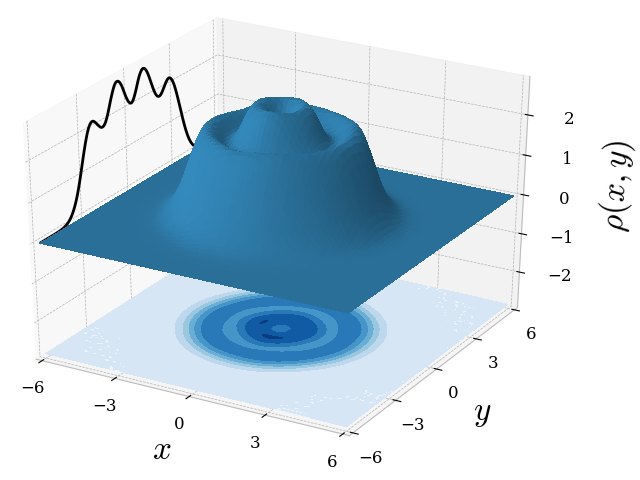
\includegraphics[width=3cm]{../plots/int1/onebody2/2D/20P/1.000000w/RBM_ADAM_MC1048576.png}}}\hspace{0.5cm}
		\subfloat{\raisebox{1cm}{\rotatebox[origin=t]{90}{RBM+SJ}}}\hspace{0.cm}
		\subfloat{{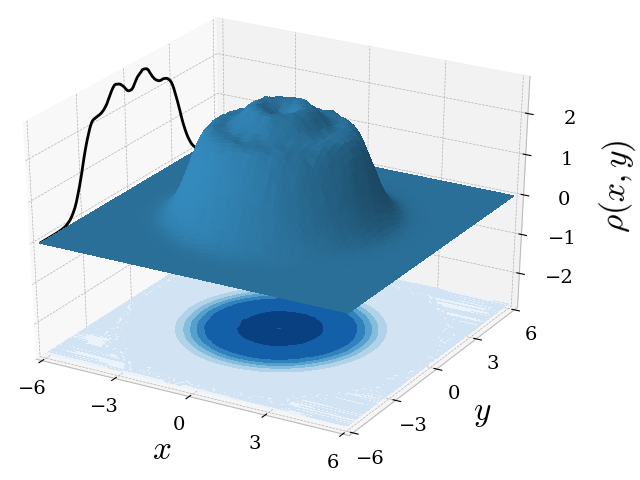
\includegraphics[width=3cm]{../plots/int1/onebody2/2D/20P/1.000000w/RBMSJ_ADAM_MC1048576.png}}}\\
		\subfloat{\raisebox{1cm}{\rotatebox[origin=t]{90}{RBM+PJ}}}\hspace{0.cm}
		\subfloat{{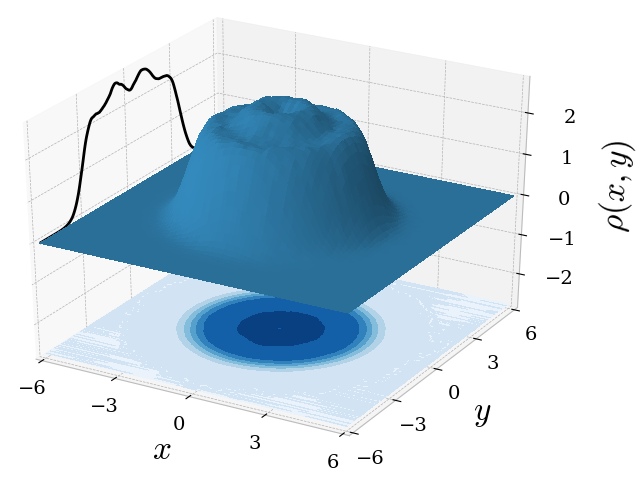
\includegraphics[width=3cm]{../plots/int1/onebody2/2D/20P/1.000000w/RBMPJ_ADAM_MC1048576.png}}}\hspace{0.5cm}
		\subfloat{\raisebox{1cm}{\rotatebox[origin=t]{90}{VMC}}}\hspace{0.cm}
		\subfloat{{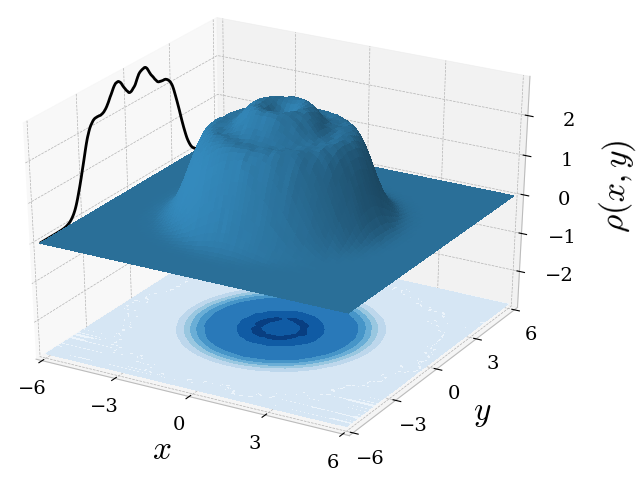
\includegraphics[width=3cm]{../plots/int1/onebody2/2D/20P/1.000000w/VMC_ADAM_MC1048576.png}}}
		
		%\caption{Plots of the one-body density profiles, $\rho(x,y)$, for two-dimensional quantum dots with $N=20$ electrons and frequency $\omega=1.0$.}%
	\end{figure}
}

\mframe{Two-body density}{
	\begin{figure}
		\centering
		\captionsetup[subfigure]{labelformat=empty}
		\subfloat{\raisebox{1cm}{\rotatebox[origin=t]{90}{RBM}}}\hspace{0.cm}
		\subfloat{{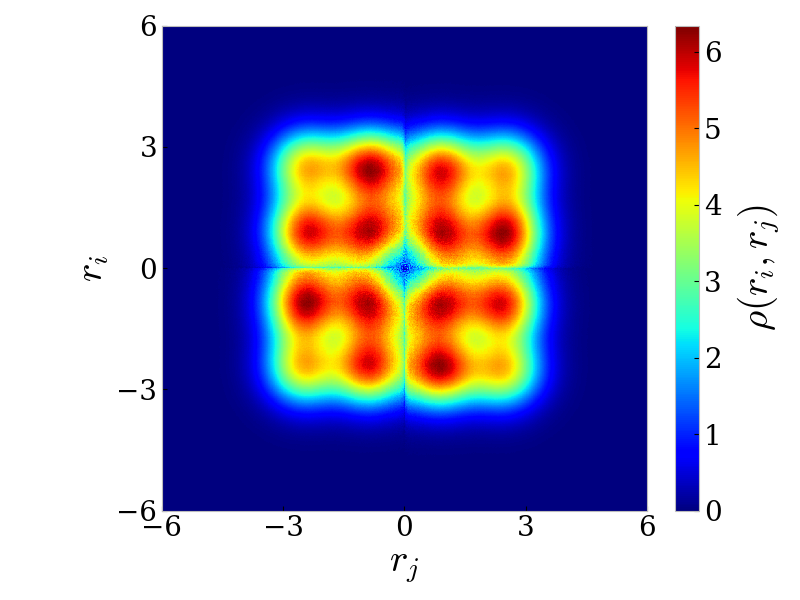
\includegraphics[width=3cm]{../plots/int1/twobody/2D/20P/1.000000w/RBM_ADAM_MC1048576.png}}}\hspace{0.5cm}
		\subfloat{\raisebox{1cm}{\rotatebox[origin=t]{90}{RBM+SJ}}}\hspace{0.cm}
		\subfloat{{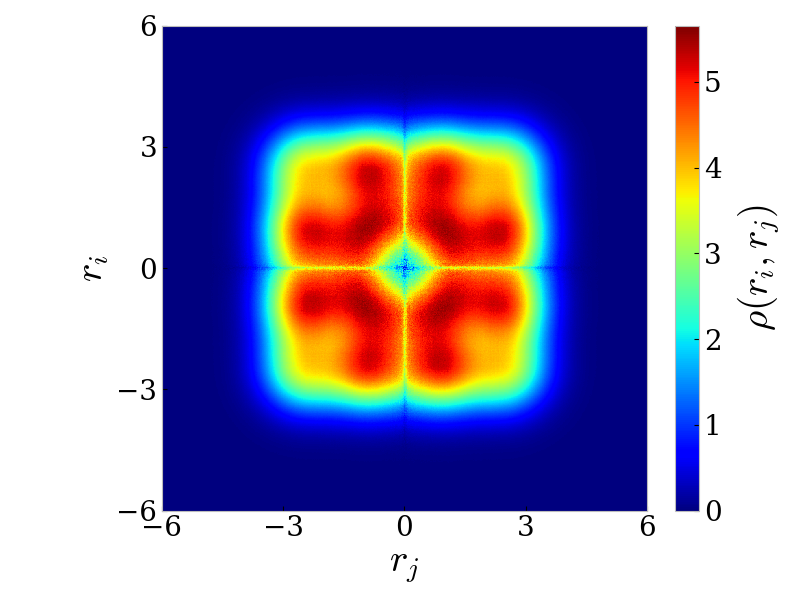
\includegraphics[width=3cm]{../plots/int1/twobody/2D/20P/1.000000w/RBMSJ_ADAM_MC1048576.png}}}\\
		\subfloat{\raisebox{1cm}{\rotatebox[origin=t]{90}{RBM+PJ}}}\hspace{0.cm}
		\subfloat{{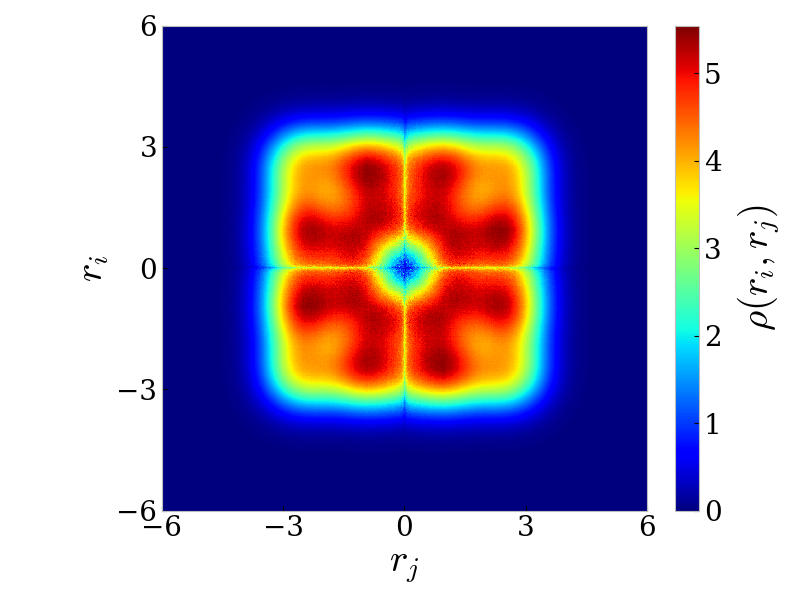
\includegraphics[width=3cm]{../plots/int1/twobody/2D/20P/1.000000w/RBMPJ_ADAM_MC1048576.png}}}\hspace{0.5cm}
		\subfloat{\raisebox{1cm}{\rotatebox[origin=t]{90}{VMC}}}\hspace{0.cm}
		\subfloat{{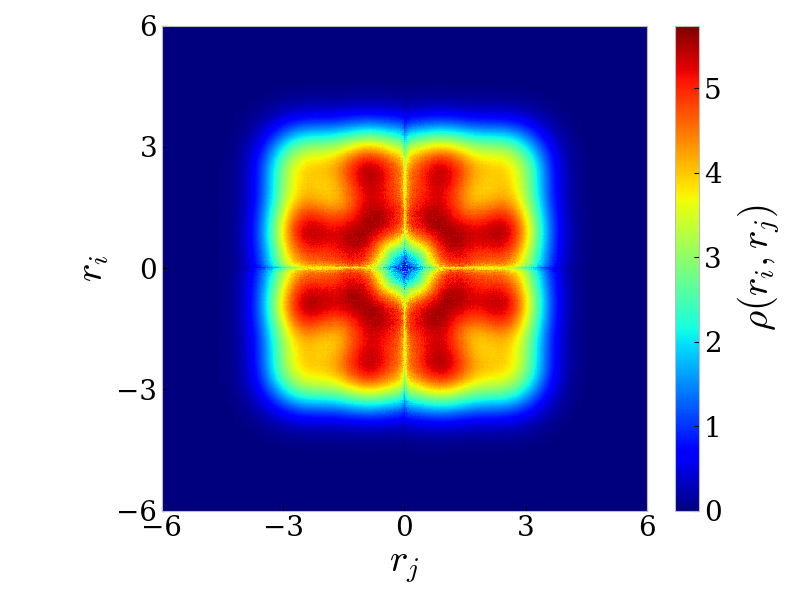
\includegraphics[width=3cm]{../plots/int1/twobody/2D/20P/1.000000w/VMC_ADAM_MC1048576.png}}}
		
		%\caption{Plots of the two-body density profiles, $\rho(r_i,r_j)$, for two-dimensional quantum dots with $N=20$ electrons and frequency $\omega=1.0$.}%
	\end{figure}
}

\mframe{Energy distribution}{
	Distribution between various energy sources
}

\mframe{Low-frequency dots}{
	\begin{figure}
		\centering
		\captionsetup[subfigure]{labelformat=empty}
		\subfloat{\raisebox{1cm}{\rotatebox[origin=t]{90}{RBM}}}\hspace{0.cm}
		\subfloat{{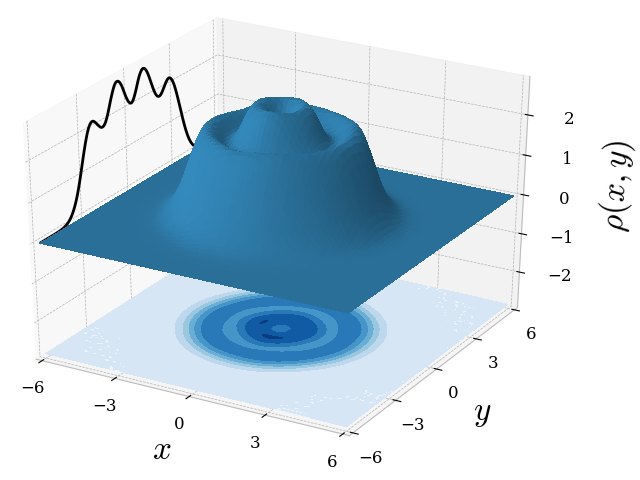
\includegraphics[width=3cm]{../plots/int1/onebody2/2D/20P/1.000000w/RBM_ADAM_MC1048576.png}}}\hspace{0.5cm}
		\subfloat{\raisebox{1cm}{\rotatebox[origin=t]{90}{RBM+SJ}}}\hspace{0.cm}
		\subfloat{{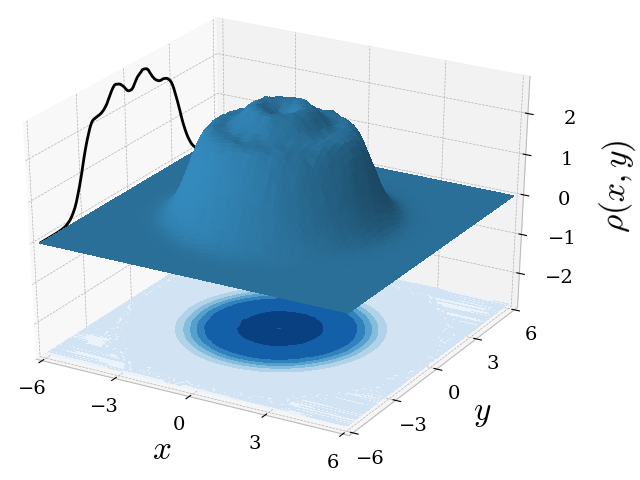
\includegraphics[width=3cm]{../plots/int1/onebody2/2D/20P/1.000000w/RBMSJ_ADAM_MC1048576.png}}}\\
		\subfloat{\raisebox{1cm}{\rotatebox[origin=t]{90}{RBM+PJ}}}\hspace{0.cm}
		\subfloat{{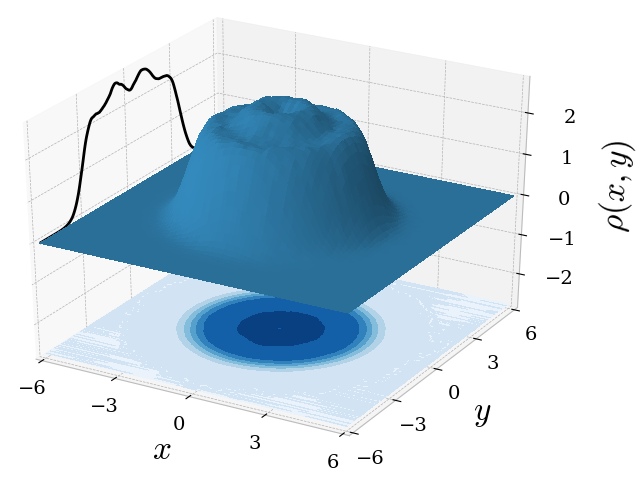
\includegraphics[width=3cm]{../plots/int1/onebody2/2D/20P/1.000000w/RBMPJ_ADAM_MC1048576.png}}}\hspace{0.5cm}
		\subfloat{\raisebox{1cm}{\rotatebox[origin=t]{90}{VMC}}}\hspace{0.cm}
		\subfloat{{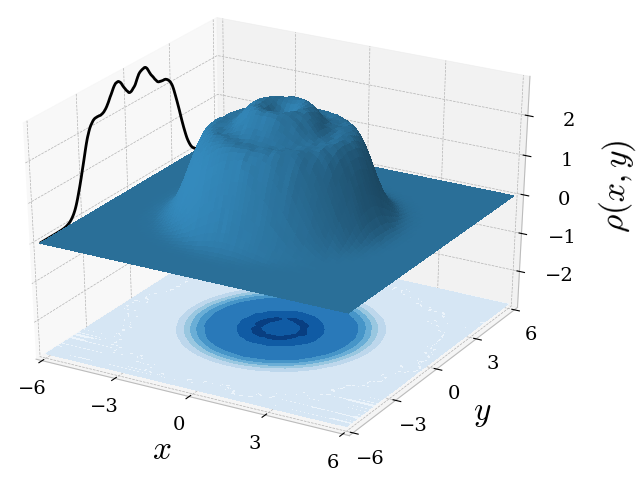
\includegraphics[width=3cm]{../plots/int1/onebody2/2D/20P/1.000000w/VMC_ADAM_MC1048576.png}}}
		
		%\caption{Plots of the one-body density profiles, $\rho(x,y)$, for two-dimensional quantum dots with $N=20$ electrons and frequency $\omega=1.0$.}%
	\end{figure}
}

\mframe{Computational Cost}{
	\begin{figure}
		\centering 
		% This file was created by matplotlib2tikz v0.7.4.
\begin{tikzpicture}[scale=0.9]

\begin{axis}[name=2D, xlabel=$N$, ylabel={CPU-time [s]}, grid=major, legend pos=north west, xtick=data] 
\addplot[color=color1,mark=oplus*, dashed] coordinates { 
	(2,6.05)
	(6,11.25)
	(12,20.53) 
	(20,38.99) 
	(30,73.73) 
	(42,130.49) 
	(56,213.47)
	(72,360.22)
	(90,856.84) }; 
\addlegendentry{RBM};

\addplot[color=color2,mark=oplus*, dash dot] coordinates { 
	(2,7.12) 
	(6,14.07) 
	(12,28.42) 
	(20,63.27) 
	(30,122.93) 
	(42,199.60)
	(56,349.22)}; 
\addlegendentry{RBM+SJ};

\addplot[color=color3,mark=oplus*, dotted] coordinates { 
	(2,7.26)
	(6,13.50)
	(12,27.68)
	(20,57.09) 
	(30,119.17) 
	(42,212.53) 
	(56,382.13) }; 
\addlegendentry{RBM+PJ};

\addplot[color=color0,mark=oplus*] coordinates { 
	(2,5.11)
	(6,10.51)
	(12,20.85) 
	(20,41.20) 
	(30,76.26) 
	(42,137.39) 
	(56,230.63)
	(72,355.81)
	(90,544.03) }; 
\addlegendentry{VMC};
\end{axis}
\end{tikzpicture}
	\end{figure} 
}

\titleframe{Conclusion}

\mframe{Conclusions}{
	\begin{itemize}
		\item RBM is able to account for most of the correlations
		\item RBM+PJ implies to give a lower ground state energy and model the correlations better than a traditional VMC
		\item RBM+SJ is both more expensive and less accurate than its fellow methods, and we see no reason to choose it
	\end{itemize}
}

\mframe{Future Work}{
	\begin{itemize}
		\item Repeat the exercise using spherical coordinates - interactions are easier to model in spherical coordinates
		\item Check the ability of modeling the three-body correlations, considering nuclear systems
		\item Reduce the computational cost
	\end{itemize}
}

\titleframe{Thank you!}

\mframe{References}{
	\tiny{\printbibliography}
}

\end{document}